\section{Introduction}
\label{sec:intro}



Large neural networks excel in many domains, but their training and fine-tuning demand extensive computation and memory~\citep{kaplan2020scaling}.
A natural approach to mitigate this cost is to replace dense weight matrices with structured ones, such as sparse \& low-rank matrices and the Fourier transform.
However, structured matrices (which can be viewed as a general form of sparsity) have not yet seen wide adoption to date, due to two main challenges.
(1) In the \textbf{end-to-end} (E2E) training setting, they have shown unfavorable efficiency--quality tradeoffs.
Model \emph{efficiency} refers how efficient these structured matrices are on modern hardware (e.g., GPUs).
Model \emph{quality} (performance on tasks) is determined by how expressive they are (e.g., can they represent commonly used transforms such as convolution or Fourier/cosine transforms that encode domain-specific knowledge).
Existing structured matrices are either not hardware-efficient, or not expressive enough.
(2) In the setting of \textbf{dense-to-sparse} (D2S) fine-tuning of pretrained models, 
a long-standing problem for most classes of structured matrices is the lack of tractable algorithms to approximate dense pretrained weight matrices~\citep{pan2012structured}.










Sparse matrices have seen advances in training deep learning models (e.g., pruning~\citep{han2015deep}, lottery tickets~\citep{frankle2018lottery}), but most work on (entrywise) sparsification focuses on reducing training or inference FLOPs, which do not necessarily map to E2E training time on modern hardware (e.g., GPUs).
In fact, most sparse training methods \emph{slow down} training in wall-clock time~\citep{gale2019state, hooker2020hardware}.
Moreover, sparse matrices are not able to represent commonly used transforms such as convolution and the Fourier transform.
Another class of structured matrices, such as Fourier, sine/cosine, Chebyshev, are used in specialized domains such as PDE solving~\citep{trefethen2000spectral} and medical imaging~\citep{hsieh2003computed}.
However, they are difficult to use in E2E training since only specific instances of these structured matrices have fast GPU implementations (e.g., FFT). Moreover, their applications requires domain expertise to hand-pick the right transforms.
Generalizations of these transforms (e.g., Toeplitz-like~\citep{sindhwani2015structured}, orthogonal polynomial transforms~\citep{driscoll1997fast}, low-displacement rank~\citep{kailath1979displacement}, quasi-separable~\citep{eidelman1999new}), though learnable, often lack efficient implementation on GPUs~\citep{thomas2018learning} for E2E training as well.
In addition, they have no known tractable algorithm to approximate a given dense matrix~\citep{pan2012structured}, making them difficult to use in D2S fine-tuning.




\textbf{E2E training.}
The technical challenge in addressing the efficiency--quality tradeoff of structured matrices is to find a parameterization that is both efficient on block-oriented hardware (e.g., GPUs) and expressive (e.g., can represent many commonly used transforms).
We propose a class of matrices called Monarch,\footnote{They are named after the monarch butterfly.} parameterized as products of two block-diagonal matrices (up to permutation), to address this challenge.
This parameterization leverages optimized batch-matrix-multiply (BMM) routines on GPUs, yielding up to 2$\times$ speedup compared to dense matrix multiply (\cref{subsec:benchmark_tasks}).
We show that the class of Monarch matrices contains the class of butterfly matrices~\citep{parker1995random,dao2019learning}, which can represent any low-depth arithmetic circuits in near optimal runtime and parameter size~\citep{dao2020kaleidoscope}.
Monarch matrices inherit this expressiveness and thus can represent many fast transforms (e.g., Fourier, sine/cosine/Chebyshev transforms, convolution) (\cref{thm:Monarch_expressiveness}).
\begin{figure}[t]
  \centering
  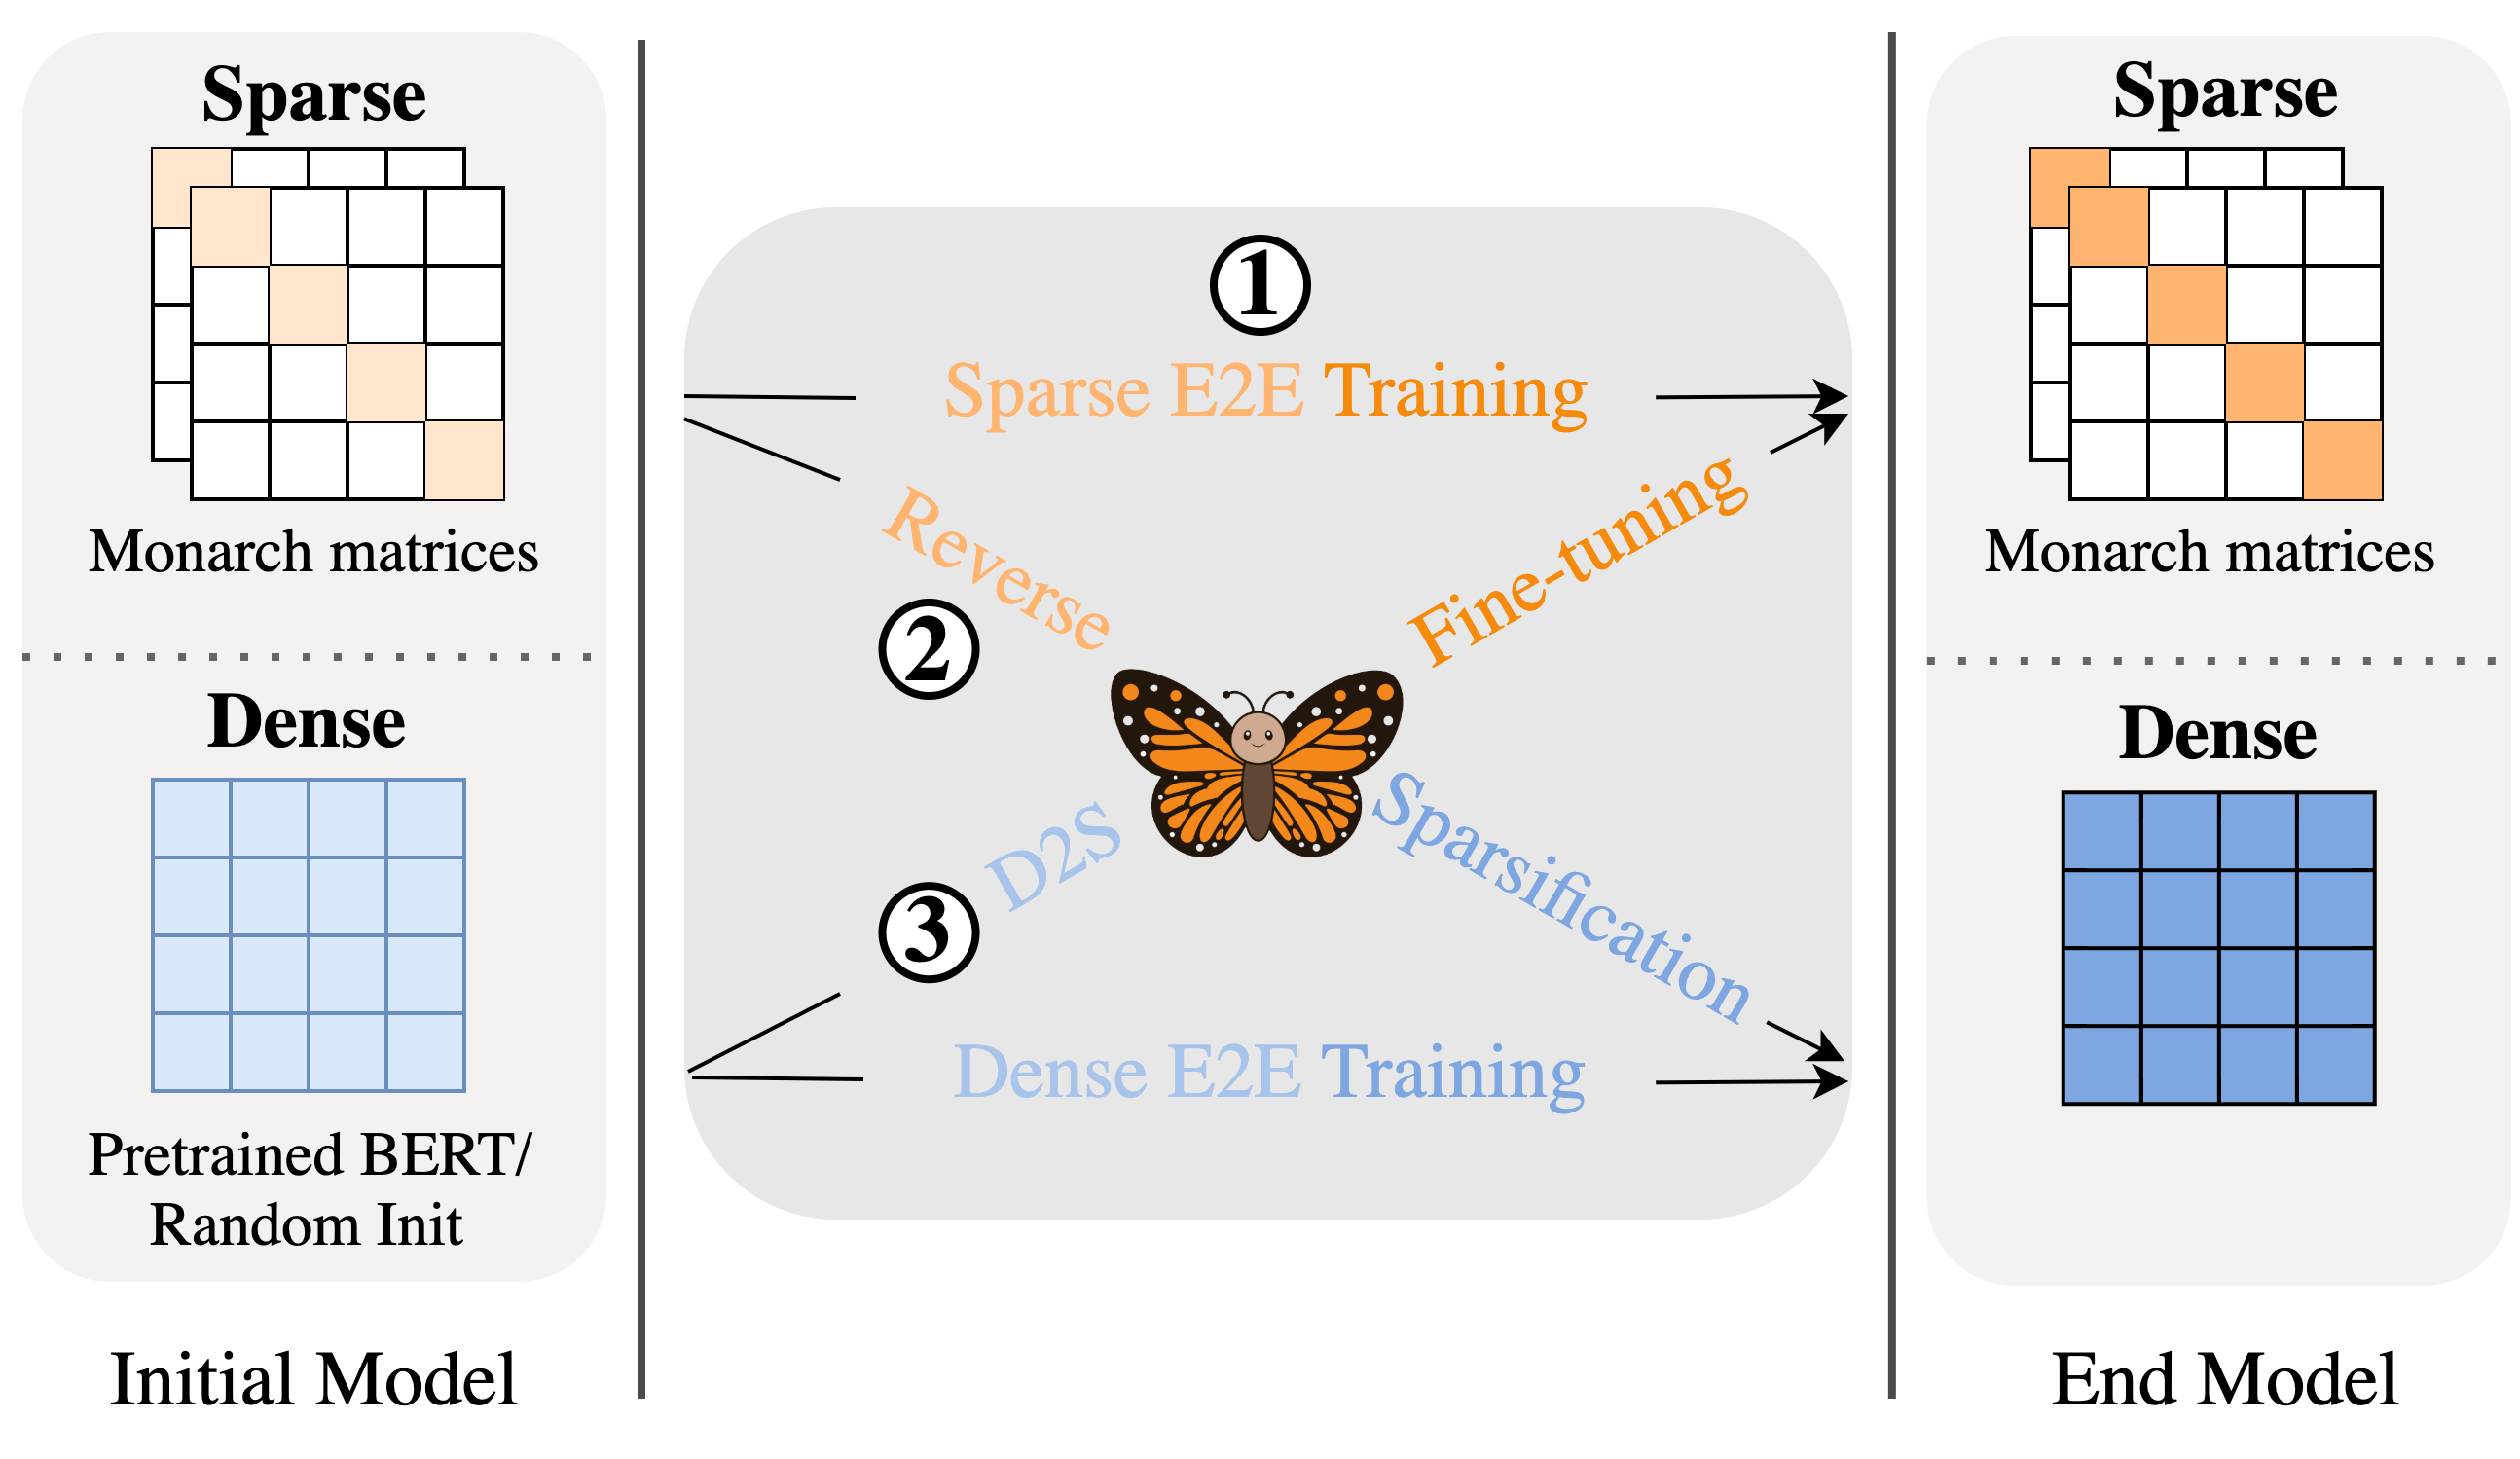
\includegraphics[width=.49\textwidth]{figures/Monarch-main.png}
  \label{fig:diagram}
  \vspace{-5mm}
  \caption{Monarch matrices unlock several ways to train sparse and dense models: end-to-end training a sparse (Monarch) model can be 2x faster than dense training thanks to its hardware efficiency; sparse-to-dense ``reverse sparsification'' can speed up training of large models such as GPT-2; and our dense-to-sparse Monarch projection algorithm can transfer knowledge from pretrained dense model to Monarch model and speed up BERT fine-tuning.}
  \vspace{-1.0em}
\end{figure}

\textbf{Sparse-to-dense (S2D) training, aka ``reverse sparsification''.} The hardware-efficiency and expressiveness of Monarch matrices unlock a new way to train dense models:
training with Monarch weight matrices for most of the time and then transitioning to dense weight matrices (\cref{fig:reverse_sparsification}).
This technique can be used in cases where sparse training faces representation or optimization difficulties~\citep{evci2019difficulty} or a dense model is necessary.
One such application is language modeling on large datasets, where a massive number of parameters are required~\citep{kaplan2020scaling} to memorize the textual patterns~\citep{geva2020transformer}.
Monarch matrices can serve as a fast intermediate representation to speed up the training process of the dense model.

\textbf{D2S fine-tuning.}
While transitioning from sparse to dense matrices is easy, the reverse direction is challenging.
The main technical difficulty is the \emph{projection} problem: finding a matrix in a class of structured matrices that is the closest to a given dense matrix.
Only a few specific classes of structured matrices have a tractable projection solution, such as entrywise sparse matrices (magnitude pruning~\citep{tewarson1973sparse}), low-rank matrices (the Eckart-Young theorem~\citep{eckart1936approximation}), and orthogonal matrices (the orthogonal Procrustes problem~\citep{schonemann1966generalized}).
For more expressive classes of structured matrices, projection remains a long-standing problem~\citep{pan2012structured}.
For example, \citet{desa2018two} show that all structured matrices (in the form of arithmetic circuits) can be written as products of sparse matrices, which can be represented as products of butterfly matrices~\citep{dao2020kaleidoscope}.
There have been numerous heuristics proposed to project on the set of butterfly matrices or products of sparse matrices, based on iterative first-order optimization~\citep{le2016flexible, dao2019learning, khalitov2021sparse} or alternating minimization~\citep{lin2021deformable}.
However, they lack theoretical guarantees.
In contrast, we derive a projection algorithm for our Monarch parameterization and prove that it finds the optimal solution (\cref{thm:Monarch_projection}).
We also derive an algorithm to factorize matrices that are products of Monarch matrices (\cref{subsec:recovery}). These new algorithms allows us to easily finetune a pretrained model into a model with Monarch weight matrices (\cref{subsec:finetuning}).







We validate our approach empirically in these three settings, showing that our Monarch matrix parameterization achieves a favorable efficiency--accuracy tradeoff compared to baselines on a wide range of domains: text, images, PDEs, MRI.
\iftoggle{arxiv}{}{
\vspace{-0.25em}
}
\begin{itemize}[leftmargin=*,nosep,nolistsep,noitemsep]
\item In the \textbf{E2E sparse training} setting (\cref{subsec:e2e_training}), our Monarch matrices model trains 2$\times$ faster than dense models while achieving the same accuracy / perplexity on benchmark tasks (ViT on ImageNet classification, GPT-2 on Wikitext-103 language modeling).
On scientific and medical tasks relying on hand-crafted fast transforms (PDE solving, MRI reconstruction), Monarch reduces the error by up to 40\% at the same training speed compared to domain-specific Fourier-based methods.
\item In the \textbf{S2D training} setting (\cref{subsec:s2d_training}), our ``reverse sparsification'' process with Monarch matrices speeds up GPT-2 pretraining on the large OpenWebText dataset by 2$\times$ compared to an optimized implementation from NVIDIA~\citep{shoeybi2019megatron}, with comparable upstream and downstream (text classification) quality.
When applied to BERT pretraining, our method is 23\% faster than the implementation from Nvidia that set the MLPerf~\citep{mattson2020mlperf} 1.1 record.
\item In the \textbf{D2S fine-tuning} setting (\cref{subsec:finetuning}), we show a proof of concept that our Monarch projection algorithm speeds up BERT fine-tuning.
We project a pretrained BERT model to a Monarch matrix model and fine-tune on GLUE, with 2$\times$ fewer parameters, 1.7$\times$ faster fine-tuning speed, and similar average GLUE accuracy as the dense model.\footnote{Monarch code is available at \url{https://github.com/HazyResearch/monarch}}
\end{itemize}

